\pdfoutput=1
\RequirePackage{fix-cm}
\documentclass[a4paper, nojss, shortnames]{jss}\usepackage[]{graphicx}\usepackage[]{color}
%% maxwidth is the original width if it is less than linewidth
%% otherwise use linewidth (to make sure the graphics do not exceed the margin)
\makeatletter
\def\maxwidth{ %
  \ifdim\Gin@nat@width>\linewidth
    \linewidth
  \else
    \Gin@nat@width
  \fi
}
\makeatother

\definecolor{fgcolor}{rgb}{0.345, 0.345, 0.345}
\newcommand{\hlnum}[1]{\textcolor[rgb]{0.686,0.059,0.569}{#1}}%
\newcommand{\hlstr}[1]{\textcolor[rgb]{0.192,0.494,0.8}{#1}}%
\newcommand{\hlcom}[1]{\textcolor[rgb]{0.678,0.584,0.686}{\textit{#1}}}%
\newcommand{\hlopt}[1]{\textcolor[rgb]{0,0,0}{#1}}%
\newcommand{\hlstd}[1]{\textcolor[rgb]{0.345,0.345,0.345}{#1}}%
\newcommand{\hlkwa}[1]{\textcolor[rgb]{0.161,0.373,0.58}{\textbf{#1}}}%
\newcommand{\hlkwb}[1]{\textcolor[rgb]{0.69,0.353,0.396}{#1}}%
\newcommand{\hlkwc}[1]{\textcolor[rgb]{0.333,0.667,0.333}{#1}}%
\newcommand{\hlkwd}[1]{\textcolor[rgb]{0.737,0.353,0.396}{\textbf{#1}}}%

\usepackage{framed}
\makeatletter
\newenvironment{kframe}{%
 \def\at@end@of@kframe{}%
 \ifinner\ifhmode%
  \def\at@end@of@kframe{\end{minipage}}%
  \begin{minipage}{\columnwidth}%
 \fi\fi%
 \def\FrameCommand##1{\hskip\@totalleftmargin \hskip-\fboxsep
 \colorbox{shadecolor}{##1}\hskip-\fboxsep
     % There is no \\@totalrightmargin, so:
     \hskip-\linewidth \hskip-\@totalleftmargin \hskip\columnwidth}%
 \MakeFramed {\advance\hsize-\width
   \@totalleftmargin\z@ \linewidth\hsize
   \@setminipage}}%
 {\par\unskip\endMakeFramed%
 \at@end@of@kframe}
\makeatother

\definecolor{shadecolor}{rgb}{.97, .97, .97}
\definecolor{messagecolor}{rgb}{0, 0, 0}
\definecolor{warningcolor}{rgb}{1, 0, 1}
\definecolor{errorcolor}{rgb}{1, 0, 0}
\newenvironment{knitrout}{}{} % an empty environment to be redefined in TeX

\usepackage{alltt}
\usepackage{amsthm}
\usepackage{graphicx}
\usepackage{amsmath, amssymb, setspace, eucal, mathrsfs}
\usepackage{subfigure}
\usepackage{pdflscape}
\usepackage{comment}
\usepackage[nonumberlist]{glossaries}
\usepackage{mathtools}
\usepackage{bbm}
\usepackage{natbib}
\usepackage[ruled, vlined]{algorithm2e}
\usepackage{hyperref}

\def\lcu{\left\{}
\def\rcu{\right\}}
\def\({\left(}
\def\){\right)}
\def\[{\left[}
\def\]{\right]}
\def\<{\left<}
\def\>{\right>}
\def\lmid{\;\middle\vert\;}

\DeclarePairedDelimiter{\ceil}{\lceil}{\rceil}
\DeclarePairedDelimiter{\floor}{\lfloor}{\rfloor}

\def\E{\mathbb{E}}
\def\P{\mathbb{P}}
\newcommand{\abs}[1]{\left| #1 \right|}
\newcommand{\eqdef}{\,{\buildrel \mathrm{def} \over =}\,}

\newcommand\commentFont[1]{\footnotesize\ttfamily{#1}}
\SetCommentSty{commentFont}

\author{Rohan Shah\\The University of Queensland, Brisbane\\Data 61 \And B. Emma Huang\\Janssen Research \& Development
}
\Plainauthor{Rohan Shah, B. Emma Huang}
\title{\pkg{mpMap2} and \pkg{mpMapInteractive2}: An R pipeline for genetic map construction}
\Plaintitle{mpMap2 and mpMapInteractive2: An R pipeline for genetic map construction}

\Abstract{
Multiparent crosses of recombinant inbred lines are now being commonly generated for major crop species. Analysis of these populations typically requires construction of a genetic map, a search for quantitative trait loci (QTL) and the imputation of underlying genotypes. These steps pose a significant computational and statistical challenge. Packages \pkg{mpMap2} and \pkg{mpMapInteractive2} provide a complete pipeline such an analysis of multi-parent populations with more than 100,000 markers. }

\Keywords{Multiparent crosses, genetic map construction, qtl mapping, \proglang{C++}, \proglang{R}}
\Plainkeywords{Network reliability, residual connectivity, Monte Carlo methods, R}

\Address{
  School of Mathematics and Physics\\
  The University of Queensland\\
  Brisbane, Australia\\
  E-mail:\\
  \email{Rohan.Shah@rohan-shah.com}\\
}
\IfFileExists{upquote.sty}{\usepackage{upquote}}{}
\begin{document}

\section{Introduction}

Multiparent recombinant inbred lines are a novel class of experimental design where the genotypes of the final progeny are mosaics of the genotypes of the $2^n$ recombinant inbred founder lines. These designs have found recent application in mice \citep{Churchill2004}, Arabadopsis \citep{Kover2009}, barley \citep{Sannemann2015}, maize, rice, tomatoes \citep{Pascual2015} and wheat \citep{Huang2012, Mackay2014}. 

Existing software able to analyze multiparent designs includes \pkg{happy}, \pkg{qtl} and \pkg{mpMap} (the previous version of \pkg{mpMap2}). Packages \pkg{happy} and \pkg{qtl} are focused on qtl mapping, and do not provide the functionality necessary for map construction. Package \pkg{mpMap} provides map construction functionality for multiparent designs, but has significant limitations. Some of these limitations are computational, such as problems analysing the large data sets currently being generated. Others are statistical, such as the inability to model finite generations of selfing and residual hetrzygosity. 

These limitations motivated the development of \pkg{mpMap2} and \pkg{mpMapInteractive2}. Our goals for \pkg{mpMap2} were
\begin{enumerate}
\item To write functionality in \proglang{C++} where required. 
\item To make use of the S4 object system, to enable easier integration of \proglang{C++} code.
\item To extend the package to biparental populations. 
\item To allow for finite generations of selfing, and therefore incorporate hetrozygous lines into the map construction process. 
\item To allow the user to asses the computational resources required for an analysis. 
\end{enumerate}

\section{Experimental designs}

We first outline the most general experimental design that we wish to be able to analyse. We have $2^n$ inbred founder lines which are combined over the first $n$ generations, resulting in a line whoose genetic material is a mosaic of the original $2^n$ founders. An example of the first $n$ generations for $n = 2$ is given in Figure \ref{fig:intercrossing_2} and for $n = 3$ in Figure \ref{fig:intercrossing_3}. 

After the first $n$ generations there is some number of generations of random intermating (possibly zero), and some number of generations of inbreeding by selfing (possibly zero). Mathematically it is possible to assume that the number of generations of inbreeding is infinite, and in this case the design is said to be a $2^n$-way RIL \citep{Teuscher2007}. Of course in practice this cannot be achieved. If the number of generations of selfing is non-zero and the number of generations of inbreeding is assumed to be infinite, the design is said to be a $2^n$-way intermated recombinant inbred population (IRIP) \citep{Teuscher2007}.

One complication is that different orders of the founders in the initial cross result in genetically different individuals at the $n$th generation. These initial crosses are known as \emph{funnels}. Accounting for symmetries, there are three different funnels for the $4$ parent design, and $315$ different funnels for the 8-parent design. Two cases are mathematically tractable. In the first, only one funnel is ever used. In the second every funnel is chosen at random, which averages out the differences between the funnels.

\begin{figure}
\centering
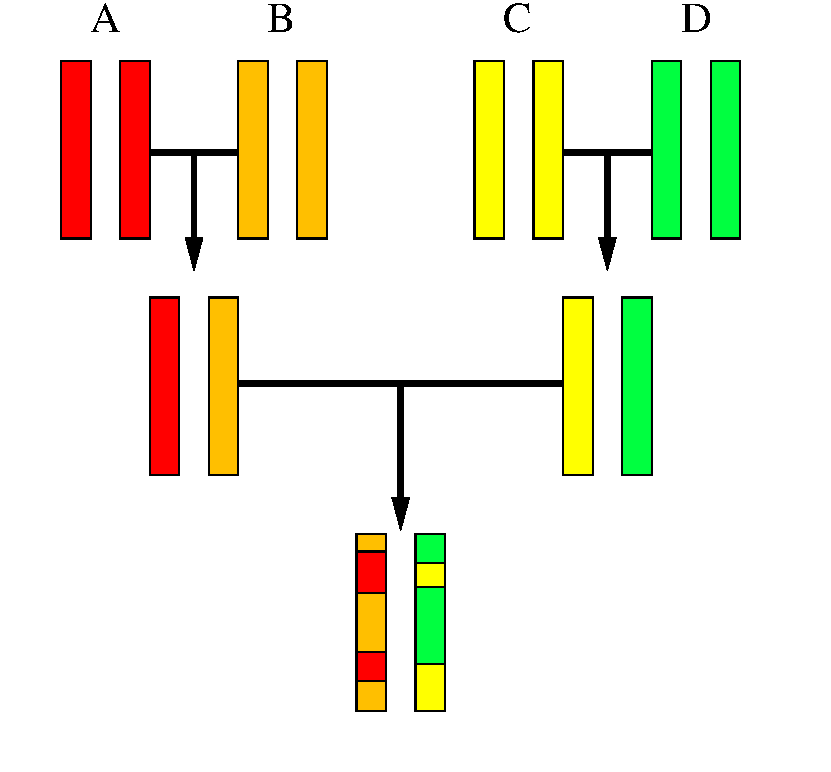
\includegraphics[width=0.35\textwidth]{MAGIC4.pdf}
\caption{Combining four founders into a single line\label{fig:intercrossing_2}}
\end{figure}

\begin{figure}
\centering
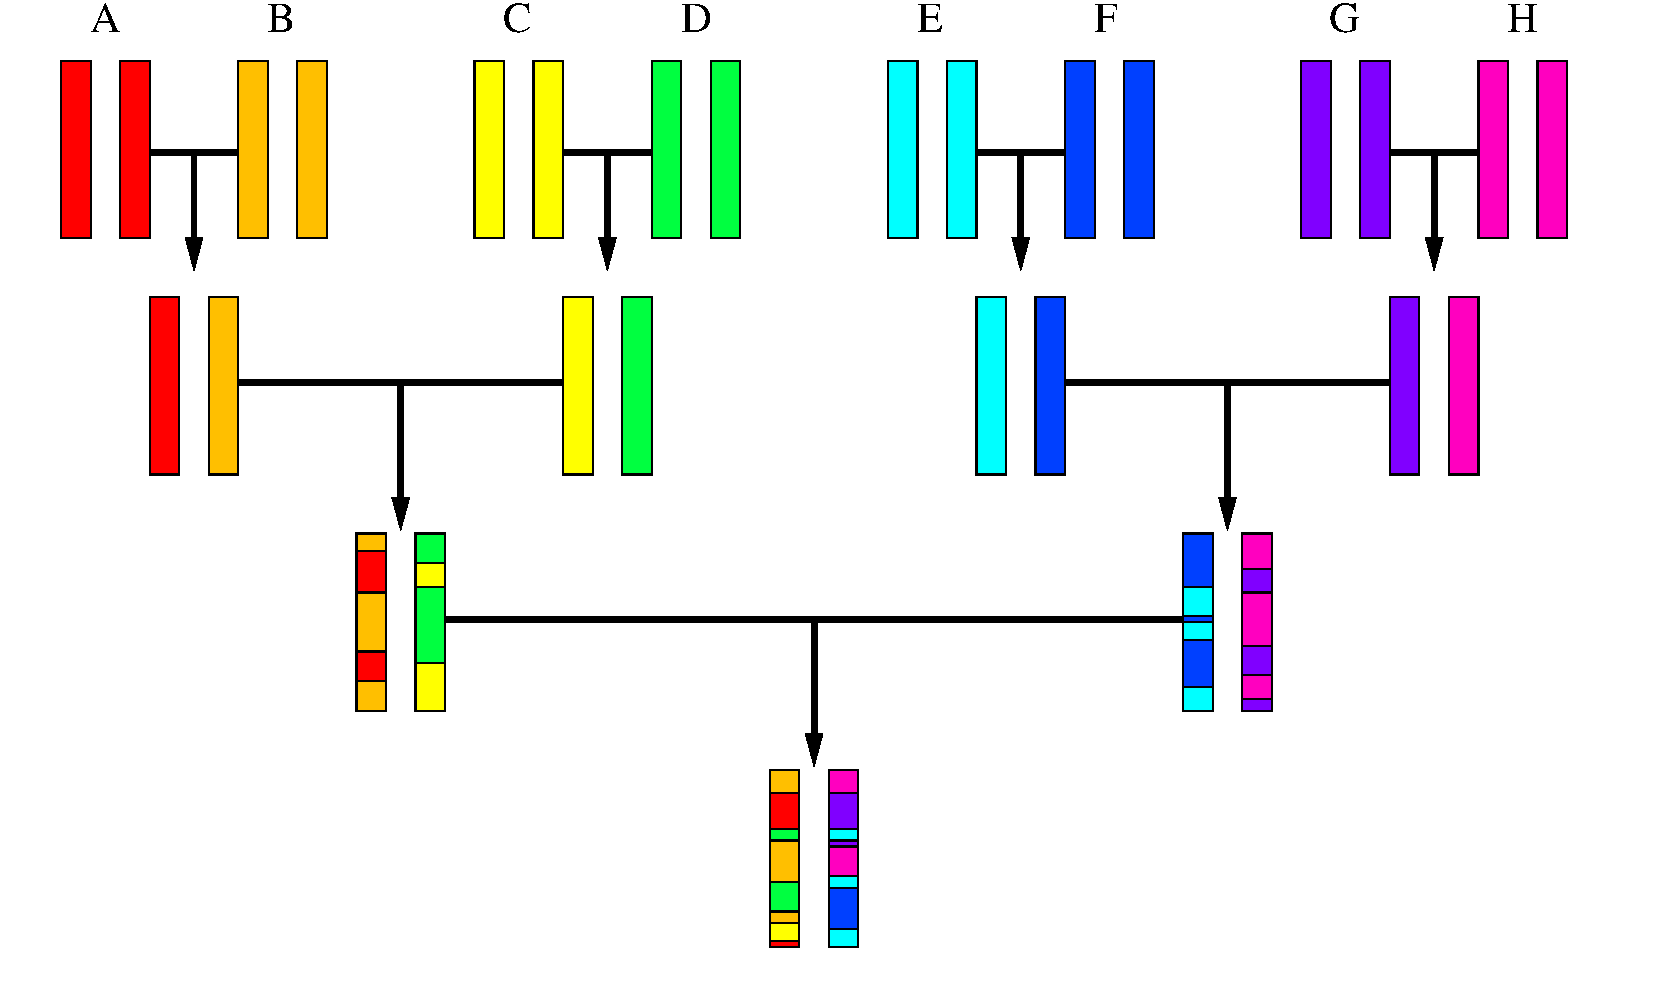
\includegraphics[width=0.8\textwidth]{MAGIC8.pdf}
\caption{Combining eight founders into a single line\label{fig:intercrossing_3}}
\end{figure}

\section{Simulation}

\subsection{Pedigrees}

Package \pkg{mpMap2} provides code for the generation of a large number of pedigrees. The two biparental design functions are \code{rilPedigree(populationSize, selfingGenerations)} which generates a biparental RIL pedigree, and \code{f2Pedigree(populationSize)} which generates an F2 population. Note that the RIL pedigree requires the specification of the number of generations of selfing, and the populations generated from this pedigree is likely to contain some residual hetrozygosity. The pedigree object has a slot \code{selfing} that controls whether this hetrozygosity is modelled in the analysis. The only possible values are \code{"auto"}, in which case hetrozygosity is explicitly modelled, or \code{"infinite"} in which case the number of generations of selfing is assumed to be inifinite. 

The functions for simulation of four parent RIL designs are \code{fourParentPedigreeSingleFunnel} and \code{fourParentPedigreeRandomFunnels}. In the first case only one of the three funnels is used. The second four-parent design uses randomly chosen funnels for each initial cross. 

\subsection{Genotypes}

\section{Estimation of recombination fractions}

\section{Construction of linkage groups}

\section{Ordering of chromosomes}

\section{Example}

\bibliography{./mpMap2}
\end{document}
